% mnras_template.tex
%
% LaTeX template for creating an MNRAS paper
%
% v3.0 released 14 May 2015
% (version numbers match those of mnras.cls)
%
% Copyright (C) Royal Astronomical Society 2015
% Authors:
% Keith T. Smith (Royal Astronomical Society)

% Change log
%
% v3.0 May 2015
%    Renamed to match the new package name
%    Version number matches mnras.cls
%    A few minor tweaks to wording
% v1.0 September 2013
%    Beta testing only - never publicly released
%    First version: a simple (ish) template for creating an MNRAS paper

%%%%%%%%%%%%%%%%%%%%%%%%%%%%%%%%%%%%%%%%%%%%%%%%%%
% Basic setup. Most papers should leave these options alone.
\documentclass[a4paper,fleqn,usenatbib]{mnras}

% MNRAS is set in Times font. If you don't have this installed (most LaTeX
% installations will be fine) or prefer the old Computer Modern fonts, comment
% out the following line
\usepackage{newtxtext,newtxmath}
% Depending on your LaTeX fonts installation, you might get better results with one of these:
%\usepackage{mathptmx}
%\usepackage{txfonts}

% Use vector fonts, so it zooms properly in on-screen viewing software
% Don't change these lines unless you know what you are doing
\usepackage[T1]{fontenc}
\usepackage{ae,aecompl}


%%%%% AUTHORS - PLACE YOUR OWN PACKAGES HERE %%%%%

% Only include extra packages if you really need them. Common packages are:
\usepackage{graphicx}	% Including figure files
\usepackage{amsmath}	% Advanced maths commands
\usepackage{amssymb}	% Extra maths symbols

%%%%%%%%%%%%%%%%%%%%%%%%%%%%%%%%%%%%%%%%%%%%%%%%%%

%%%%% AUTHORS - PLACE YOUR OWN COMMANDS HERE %%%%%

% Please keep new commands to a minimum, and use \newcommand not \def to avoid
% overwriting existing commands. Example:
%\newcommand{\pcm}{\,cm$^{-2}$}	% per cm-squared

\newcommand{\Msun}{\mathrm{M_{\sun}}}

%%%%%%%%%%%%%%%%%%%%%%%%%%%%%%%%%%%%%%%%%%%%%%%%%%

%%%%%%%%%%%%%%%%%%% TITLE PAGE %%%%%%%%%%%%%%%%%%%

% Title of the paper, and the short title which is used in the headers.
% Keep the title short and informative.
\title[]{Insert clever, witty title here}

% The list of authors, and the short list which is used in the headers.
% If you need two or more lines of authors, add an extra line using \newauthor
\author[I.D. Roberts \& L.C. Parker]{
Ian D. Roberts,\thanks{E-mail: roberid@mcmaster.ca}
Laura C. Parker
\\
% List of institutions
Department of Physics and Astronomy, McMaster University, Hamilton ON
L8S 4M1, Canada
}

% These dates will be filled out by the publisher
\date{Accepted XXX. Received YYY; in original form ZZZ}

% Enter the current year, for the copyright statements etc.
\pubyear{2016}

% Don't change these lines
\begin{document}
\label{firstpage}
\pagerange{\pageref{firstpage}--\pageref{lastpage}}
\maketitle

% Abstract of the paper
\begin{abstract}
\end{abstract}

% Select between one and six entries from the list of approved keywords.
% Don't make up new ones.
\begin{keywords}
galaxies: clusters: general -- galaxies: evolution -- galaxies:
groups: -- galaxies: statistics
\end{keywords}

%%%%%%%%%%%%%%%%%%%%%%%%%%%%%%%%%%%%%%%%%%%%%%%%%%

%%%%%%%%%%%%%%%%% BODY OF PAPER %%%%%%%%%%%%%%%%%%

\section{Introduction}
\label{sec:introduction}

%%%%%%%%%%%%%%%%%%%%%%%%%%%%%%%%%%%%%%%%

\section{Data}
\label{sec:data}

\subsection{Yang group catalogue}

\subsection{Group dynamics}

\subsection{Matched data set}

\begin{figure}
  \centering
  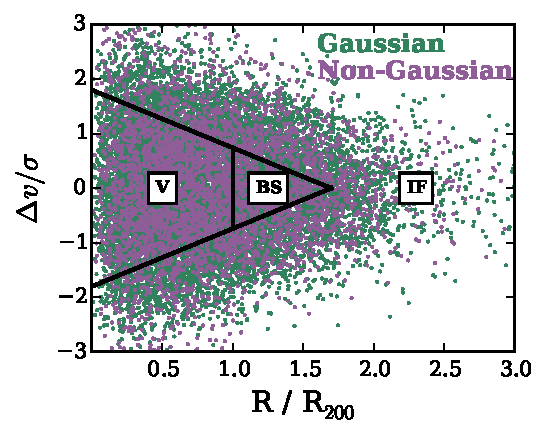
\includegraphics[width=\columnwidth]{vnorm_r.pdf}
  \caption{}
  \label{fig:vnorm_r}
\end{figure}

%%%%%%%%%%%%%%%%%%%%%%%%%%%%%%%%%%%%%%%%%%%%

\section{Results}
\label{sec:results}

\subsection{Infalling region}

\begin{figure}
  \centering
  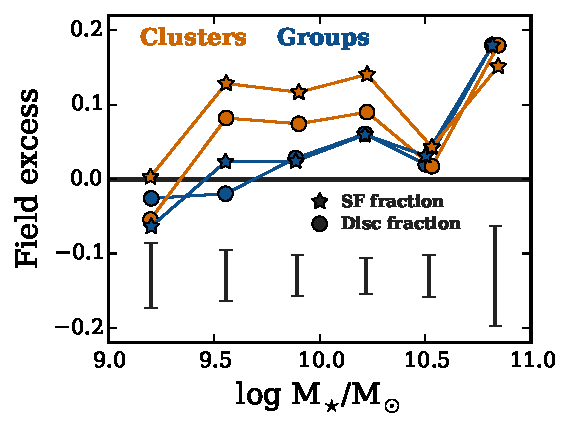
\includegraphics[width=\columnwidth]{mh_excess.pdf}
  \caption{}
  \label{fig:mh_excess}
\end{figure}

\subsection{Virialized region}

%%%%%%%%%%%%%%%%%%%%%%%%%%%%%%%%%%%%%%%%%%%

\section{Discussion}
\label{sec:discussion}

%%%%%%%%%%%%%%%%%%%%%%%%%%%%%%%%%%%%%%%%%%%

\section{Summary \& conclusions}
\label{sec:summary} 

%%%%%%%%%%%%%%%%%%%%%%%%%%%%%%%%%%%%%%%%%%

\section*{Acknowledgments}
\label{sec:acknowledgments}

IDR thanks the Ontario Graduate Scholarship program for funding.  LCP
thanks the National Science and Engineering Research
Council of Canada for funding.  The authors thank
F. Evans for matching together the various SDSS catalogues used in
this research.  We thank X. Yang et al. for
making their
SDSS DR7 group catalogue publicly available, L. Simard et al. for the
publication of their SDSS DR7 morphology catalogue, J. Brinchmann et al. for
publication of their SDSS SFRs, and the NYU-VAGC
team for the 
publication of their SDSS DR7 catalogue.  This research would not have
been possible without access to these public catalogues.
\par
Funding for the SDSS has been provided by the Alfred P. Sloan
Foundation, the Participating Institutions, the National Science
Foundation, the U.S. Department of Energy, the National Aeronautics
and Space Administration, the Japanese Monbukagakusho, the Max Planck
Society, and the Higher Education Funding Council for England. The
SDSS Web Site is http://www.sdss.org/.
\par
The SDSS is managed by the Astrophysical Research Consortium for the
Participating Institutions. The Participating Institutions are the
American Museum of Natural History, Astrophysical Institute Potsdam,
University of Basel, University of Cambridge, Case Western Reserve
University, University of Chicago, Drexel University, Fermilab, the
Institute for Advanced Study, the Japan Participation Group, Johns
Hopkins University, the Joint Institute for Nuclear Astrophysics, the
Kavli Institute for Particle Astrophysics and Cosmology, the Korean
Scientist Group, the Chinese Academy of Sciences (LAMOST), Los Alamos
National Laboratory, the Max-Planck-Institute for Astronomy (MPIA),
the Max-Planck-Institute for Astrophysics (MPA), New Mexico State
University, Ohio State University, University of Pittsburgh,
University of Portsmouth, Princeton University, the United States
Naval Observatory, and the University of Washington.

%%%%%%%%%%%%%%%%%%%%%%%%%%%%%%%%%%%%%%%%%%%%%%%%%%

%%%%%%%%%%%%%%%%%%%% REFERENCES %%%%%%%%%%%%%%%%%%

% The best way to enter references is to use BibTeX:

\bibliographystyle{mnras}
\bibliography{RobertsParker2016} % if your bibtex file is called example.bib


% Alternatively you could enter them by hand, like this:
% This method is tedious and prone to error if you have lots of references
%\begin{thebibliography}{99}
%\bibitem[\protect\citeauthoryear{Author}{2012}]{Author2012}
%Author A.~N., 2013, Journal of Improbable Astronomy, 1, 1
%\bibitem[\protect\citeauthoryear{Others}{2013}]{Others2013}
%Others S., 2012, Journal of Interesting Stuff, 17, 198
%\end{thebibliography}


% Don't change these lines
\bsp	% typesetting comment
\label{lastpage}
\end{document}

% End of mnras_template.tex
